\section{Red a analizar}

De cara a realizar esta práctica se va a analizar la red de seguidores de la Escuela Técnica Superior de Ingenierías Informática y de Telecomunicación (ETSIIT), de la Universidad de Granada.

He escogido esta red ya que me parece interesante estudiar las conexiones que puede tener la ETSIIT al ser un centro donde coinciden distintos perfiles, investigadores, estudiantes, docentes, empresas, instituciones, etc, lo que puede ser interesante ver y comprender como interactúan todo este tipo de perfiles, y observar si es fácil hacer estas distinciones entre perfiles.

\subsection{Obtención de los datos de la red}

Para obtener los datos de los seguidores de Twitter he utilizado la herramienta twitter-graph \cite{twitterGraph}. Esta herramienta permite utilizar nuestras credenciales de desarrollador de Twitter para realizar peticiones a la API de Twitter, como obtener los seguidores y conexiones de cierto usuario, buscar por términos concretos en todo Twitter, o obtener los me gusta a los que le ha dado un usuario.

En nuestro caso se ha utilizado para obtener los datos de los seguidores de la cuenta de la ETSIIT \cite{twitterETSIIT}. Al utilizar esta herramienta se nos ha generado dos ficheros csv, uno con los datos de los nodos y otro con la información de los enlaces.

\subsection{Previsualización de toda la red}

Una vez exportamos los datos a Gephi, podemos visualizar la red. De cara a poder visualizarla sin perder resolución, se ha exportado como PDF y se ha incrustado la página obtenida en esta memoria. Se ha utilizado el algoritmo ForceAtlas 2 para visualización, intentando que la red quede lo más estética posible, pero como vamos a ver se trata de una red muy densa, donde existen muchas conexiones y no es sencillo hacer un primer análisis visual claro.

Esta visualización es la generada directamente por Gephi, por lo que podemos hacer zoom a dicha visualización para poder ver en detalle la red.

\newpage
\begin{figure}[H]
	\centering
	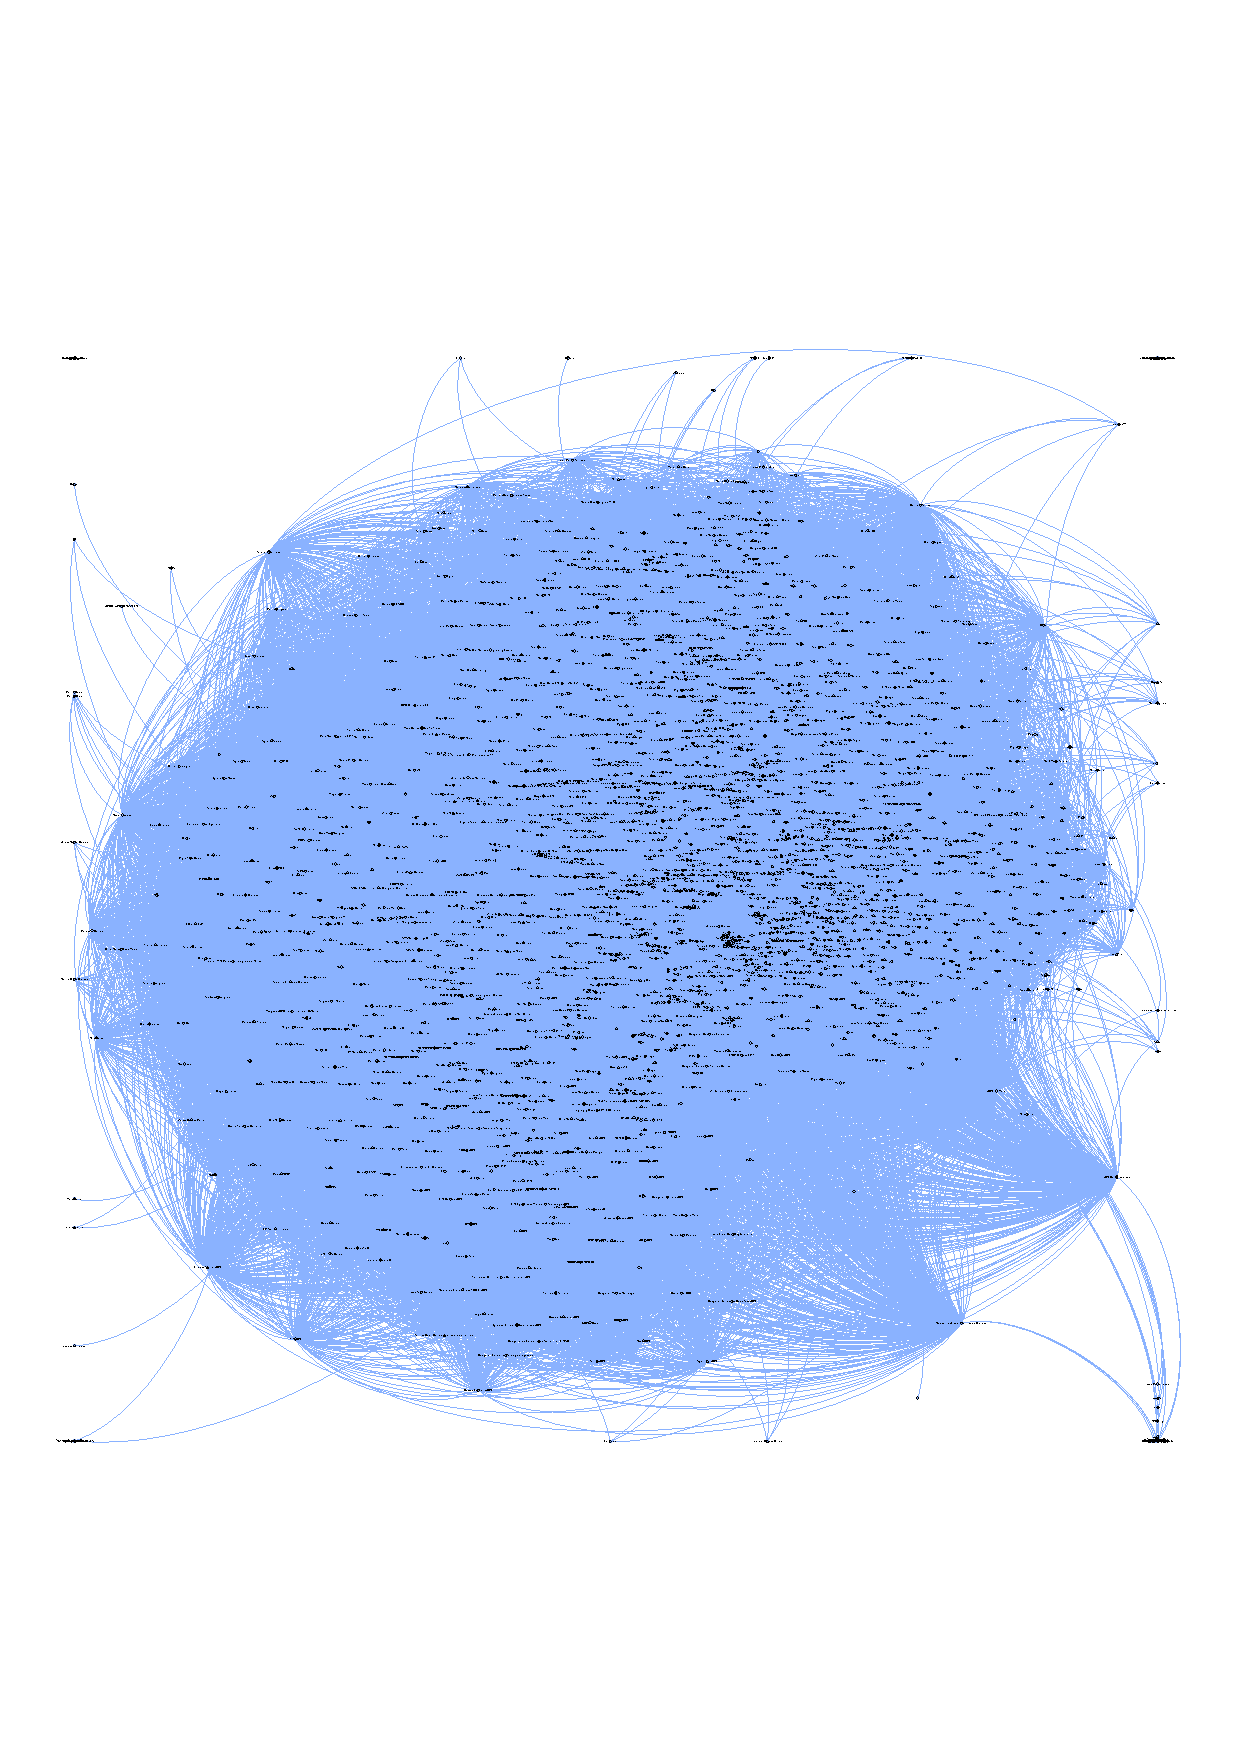
\includepdf[frame=true, scale=0.9, offset=75 -50]{pdf_incrustados/red_completa.pdf}
	\caption{Red completa de seguidores de la cuenta ETSIIT}
\end{figure}
\newpage


\subsection{Previsualización de la componente gigante de la red}

Con Gephi podemos observar el número de componentes conexos de la red, que en este caso son 65. Como podemos ver en el informe generado por Gephi, 64 de estas son nodos sin conexiones y la componente gigante contiene la mayor parte de los nodos y todas las conexiones:


\begin{figure}[H]
  \centering
  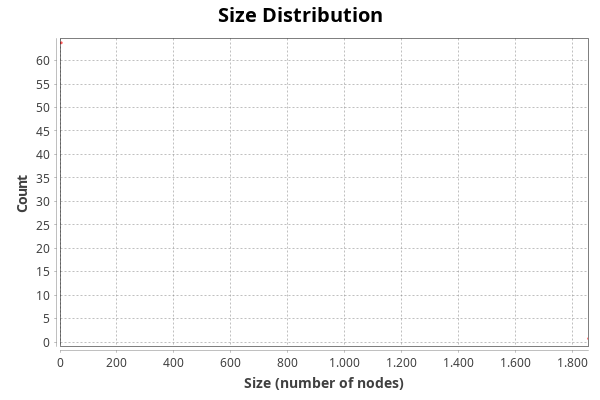
\includegraphics[width = \textwidth]{componentes_conexos.png}
  \caption{Informe sobre componentes conexos de Gephi sobre la red de seguidores de la ETSIIT.}
  \label{fig:componentes_conexos}
\end{figure}

Vamos a visualizar la red únicamente con la componente gigante, que como veremos, no aparecerán los nodos en los extremos que podíamos ver en la red completa.

\newpage
\begin{figure}[H]
	\centering
	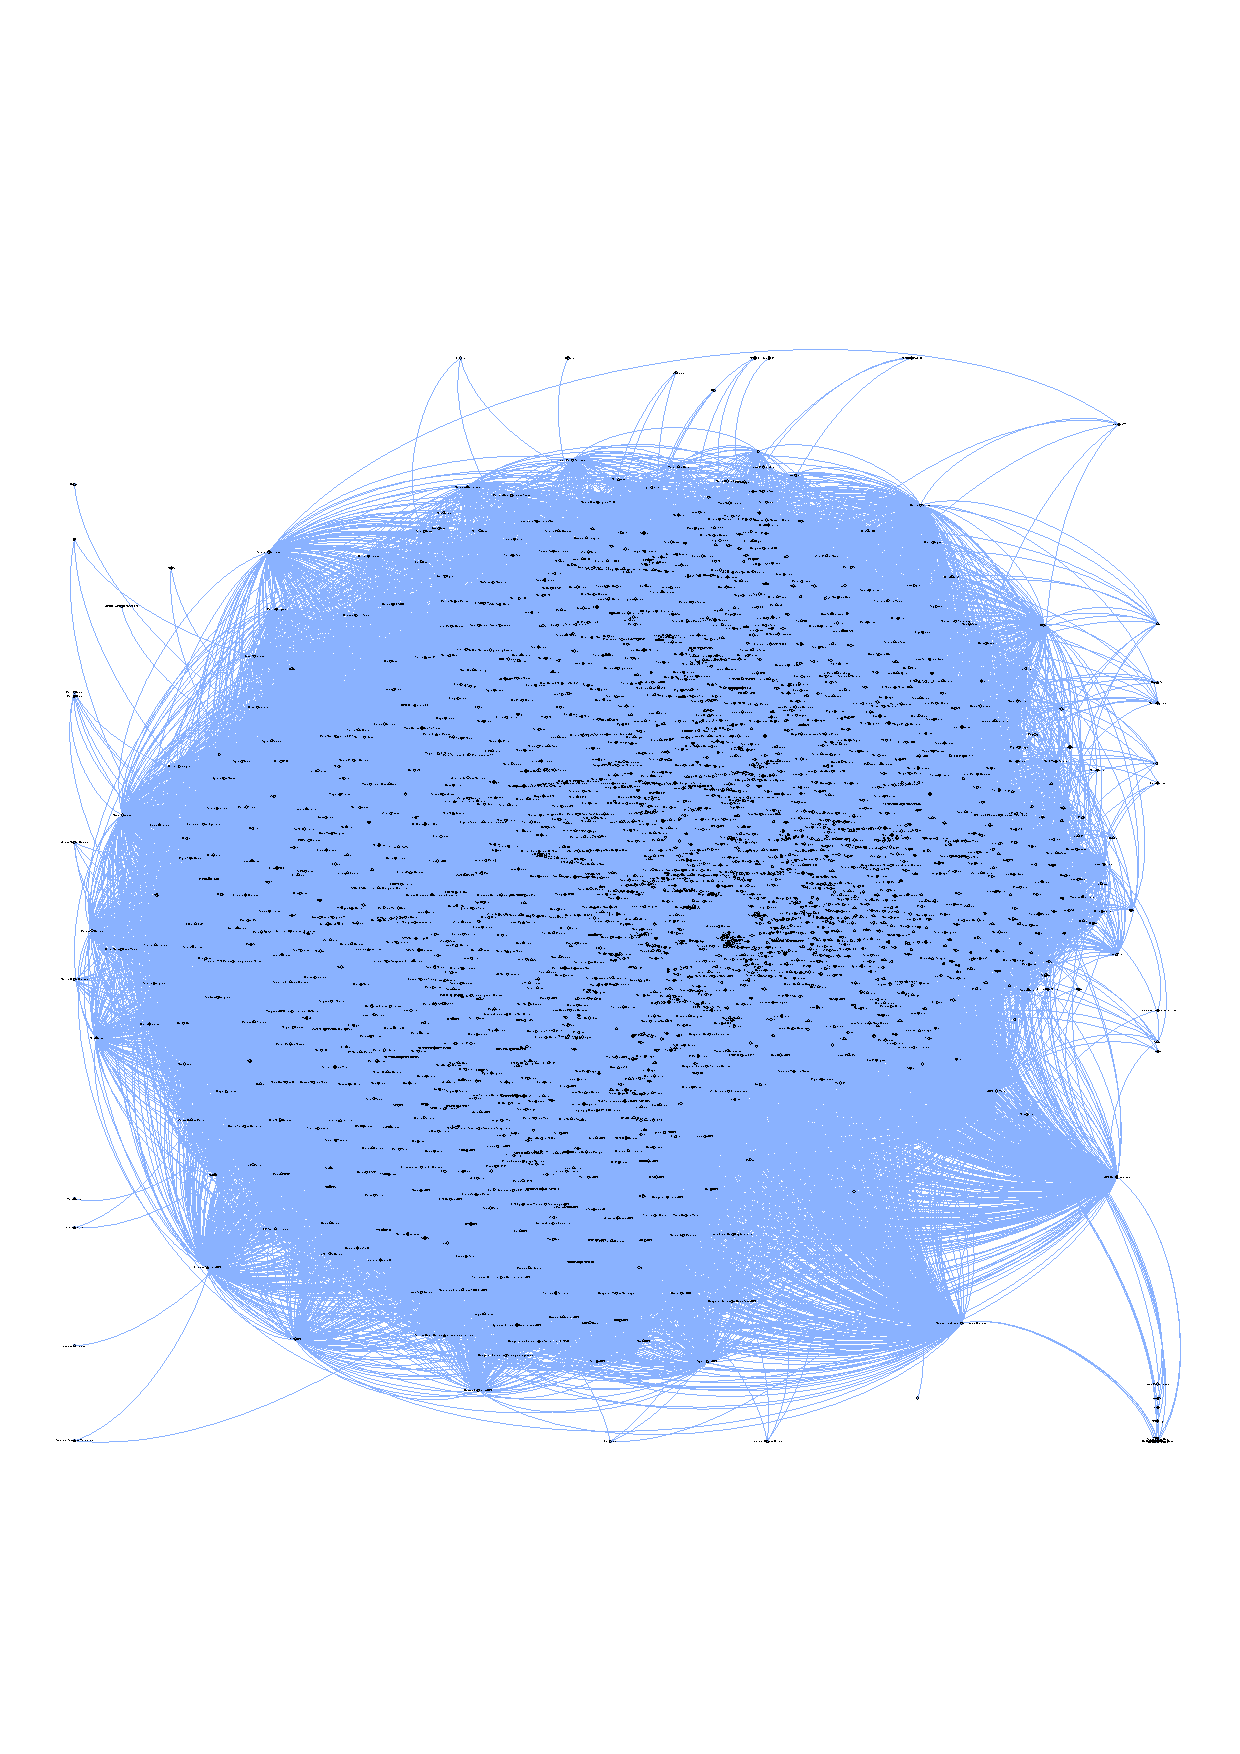
\includepdf[frame=true, scale=0.9, offset=75 -50]{pdf_incrustados/componente_gigante.pdf}
	\caption{Componente gigante de seguidores de la cuenta ETSIIT}
\end{figure}
\newpage

\subsection{Medidas de la red}

Como se pedía en el guión de prácticas, también se ha obtenido diversas medidas estadísticas sobre la red:

% Please add the following required packages to your document preamble:
% \usepackage{graphicx}
\begin{table}[H]
\centering
\begin{tabular}{|l|r|}
\hline
\multicolumn{1}{|c|}{\textbf{Medida}}                      & \multicolumn{1}{c|}{\textbf{Valor}} \\ \hline
Número de nodos N                                          & 1916                                \\ \hline
Número de enlaces L                                        & 47334                               \\ \hline
Número máximo de enlaces Lmax                              & 3.669.140                           \\ \hline
Densidad del grafo L/Lmax                                  & 0,013                               \\ \hline
Grado medio \textless{}k\textgreater{}                     & 24,705                              \\ \hline
Diámetro dmax                                              & 7                                   \\ \hline
Distancia media d                                          & 2,598965954                         \\ \hline
Coeficiente medio de clustering \textless{}C\textgreater{} & 0,407                               \\ \hline
Número de componentes conexas                              & 65                                  \\ \hline
Número de nodos componente gigante (y \%)                  & 1852 (0,966)                        \\ \hline
Número de aristas componente gigante (y \%)                & 47334 (1)                           \\ \hline
Diámetro dmax componente gigante                           & 7                                   \\ \hline
Distancia media d componente gigante                       & 2,598965954                         \\ \hline
\end{tabular}%
\caption{Medidas estadísticas de la red de seguidores de la ETSIIT}
\end{table}

\subsection{Gráficos sobre las medidas de la red}
